%% 美赛模板:正文部分

\documentclass[12pt]{article}  % 官方要求字号不小于 12 号,此处选择 12 号字体
\usepackage{float}
\usepackage{graphicx}
\usepackage{caption}
\usepackage{subcaption}
\usepackage{listings}
\usepackage{xcolor}
% 本模板不需要填写年份,以当前电脑时间自动生成
% 请在以下的方括号中填写队伍控制号
\usepackage[2021054]{easymcm}  % 载入 EasyMCM 模板文件
\problem{C}  % 请在此处填写题号
\usepackage{mathptmx}  % 这是 Times 字体,中规中矩 
%\usepackage{mathpazo}  % 这是 COMAP 官方杂志采用的更好看的 Palatino 字体,可替代以上的 mathptmx 宏包

\title{An MCM Paper Made by Team 1234567}  % 标题

% 如需要修改题头(默认为 MCM/ICM),请使用以下命令(此处修改为 MCM)
%\renewcommand{\contest}{MCM}

% 文档开始
\begin{document}

% 此处填写摘要内容
\begin{abstract}
    Here is the abstract of your paper.

    Firstly, that is ...

    Secondly, that is ...

    Finally, that is ...

    % 美赛论文中无需注明关键字。若您一定要使用,
    % 请将以下两行的注释号 '%' 去除,以使其生效
    % \vspace{5pt}
    % \textbf{Keywords}: MATLAB, mathematics, LaTeX.

\end{abstract}

\maketitle  % 生成 Summary Sheet
\tableofcontents  % 生成目录


% 正文开始
\section{Introduction}
\subsection{Problem Background}
Here is the problem background ...

Two major problems are discussed in this paper, which are:
\begin{itemize}
    \item Doing the first thing.
    \item Doing the second thing.
\end{itemize}

\subsection{Literature Review}
A literatrue\cite{1} say something about this problem ...

\subsection{Our work}
We do such things ...

\begin{enumerate}[\bfseries 1.]
    \item We do ...
    \item We do ...
    \item We do ...
\end{enumerate}

\section{Preparation of the Models}
\subsection{Assumptions}

\subsection{Notations}
The primary notations used in this paper are listed in Table \ref{tb:notation}.
\begin{table}[!htbp]
\begin{center}
\caption{Notations}
\begin{tabular}{cl}
	\toprule
	\multicolumn{1}{m{3cm}}{\centering Symbol}
	&\multicolumn{1}{m{8cm}}{\centering Definition}\\
	\midrule
	$A$&the first one\\
	$b$&the second one\\
	$\alpha$ &the last one\\
	\bottomrule
\end{tabular}\label{tb:notation}
\end{center}
\end{table}

\section{The Models}
\subsection{The subjectivity and polarity of a customer's review}
We assumed that each word, in the customers' reviews, has 2 properties: \textbf{subjectivity} and \textbf{polarity}. Subjective $s_{word}$ describes in what degree the word is subjective, ranges from 0 to 1. The higher $s_{word}$ is, the more subjective a word is. Polarity $p_{word}$ describes how much the customer loves or hates the product when writing the word, ranges from -1 to 1. We then define the subjectivity and the polarity of a sentences $s_{sentence}$ and $p_{sentence}$, which is the average of all the words in a sentences. Assume the number of words in a sentence is $n$, then
\begin{equation*}
  \begin{aligned}
    s_{sentence} = \dfrac{\sum\limits_{n} s_{word}}{n}  \\
    p_{sentence} = \dfrac{\sum\limits_{n} p_{word}}{n} 
  \end{aligned}
\end{equation*}
Apparently, if a customer A used 1 sentence to praise a product, and customer B used 10 sentences to praise it, customer B loves it more. So we sum up all the subjectivity and polarity of the sentences in customer's review, to indicate how subjective the customer is, and in what degree the customer loves or hates the product.
\begin{equation*}
  \begin{aligned}
    s_{customer} = \sum s_{sentence} \\
    p_{customer} = \sum p_{sentence}
  \end{aligned}
\end{equation*}
To solve this problem, of course we need a word list to store the subjectivity and polarity of different words. Perhaps we need machine learning. But in solving this problem, we didn't reinvent wheels because the wheel we invented probably won't better than the wheels in open source communities. So we used \textbf{textblob} , a python module, to calculate the subjectivity and polarity of the customers.

\subsection{The relation between rating levels and customer reviews}

To find the relation between rating levels and customer reviews, first we need to convert customer reviews, which is text based information, to numeric numbers. As we said in the previous section, we calculated the subjectivity and polarity of each customer, according to their reviews. And we used the \textbf{Curve Fitting} app in \textbf{MATLAB}, trying to fit a curve.
We imported the subjectivity, polarity and star ratings data of all the 3 products separately into \textbf{MATLAB}, and plotted the data. Then we could see from the graph that the polarity seemed to be linearly dependent with star rating, and the polarity is not dependent with star rating.
Then we used Linear Method to fit the data. These following graphs shows the relation between polarity, subjectivity and star rating of the 3 different products.
\begin{figure}[H]
  \centering
  \begin{subfigure}{.5\textwidth}
    \centering
    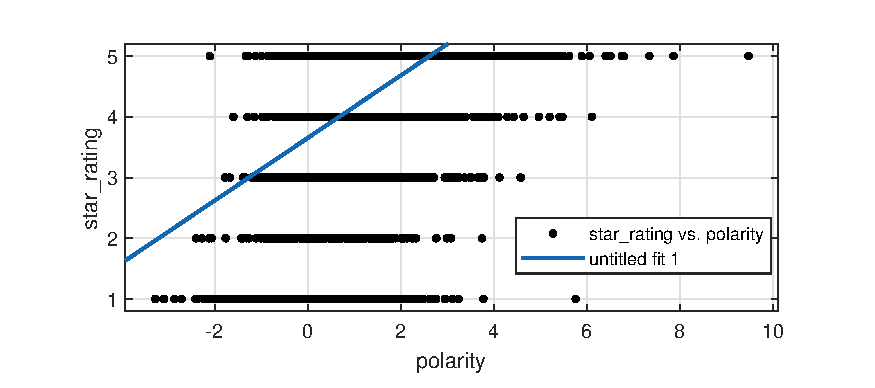
\includegraphics[width=\linewidth]{figures/hair_dryer/polarity_vs_star_rating.eps}
    \caption{star rating vs polarity}
    \label{fig:}
  \end{subfigure}%
  \begin{subfigure}{.5\textwidth}
    \centering
    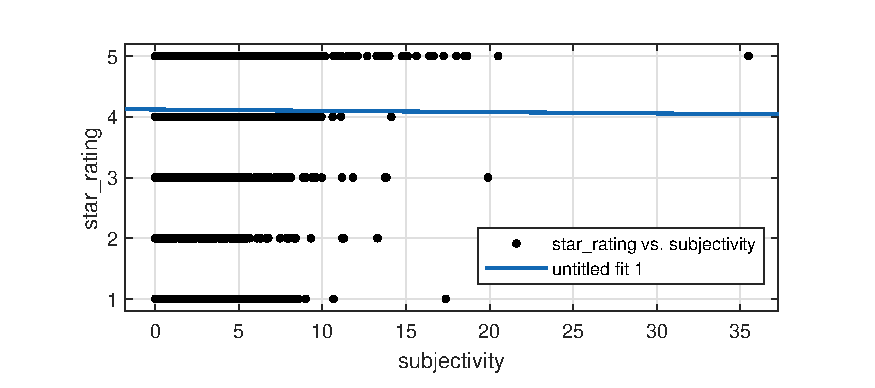
\includegraphics[width=\linewidth]{figures/hair_dryer/subjectivity_vs_star_rating.eps}
    \caption{star rating vs subjectivity}
    \label{fig:}
  \end{subfigure}
  \caption{the relation between polarity, subjectivity and star rating of the hair dryer}
  \label{fig:}
\end{figure}
\begin{figure}[H]
  \centering
  \begin{subfigure}{.5\textwidth}
    \centering
    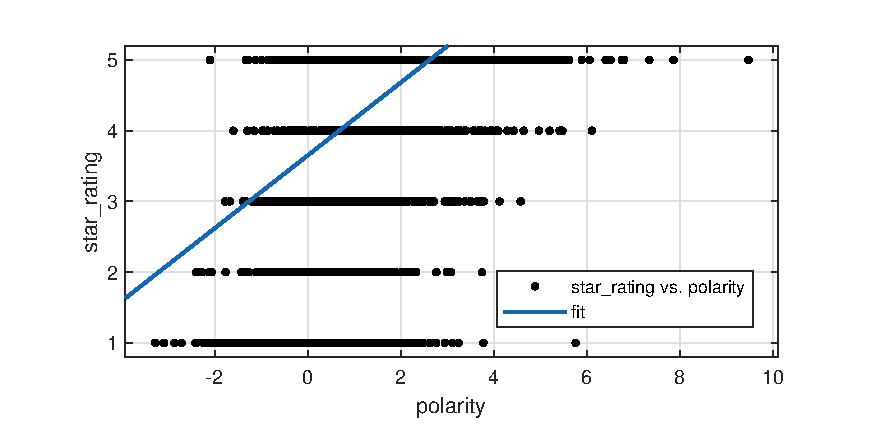
\includegraphics[width=\linewidth]{figures/microwave/polarity_vs_star_rating.eps}
    \caption{star rating vs polarity}
    \label{fig:}
  \end{subfigure}%
  \begin{subfigure}{.5\textwidth}
    \centering
    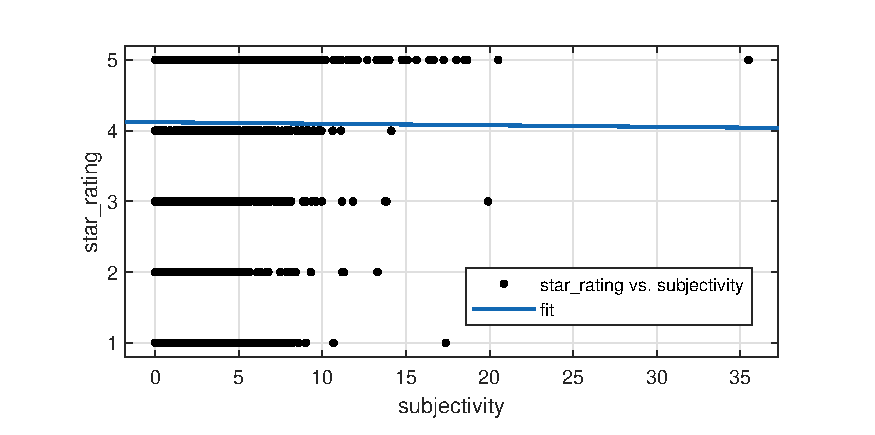
\includegraphics[width=\linewidth]{figures/microwave/subjectivity_vs_star_rating.eps}
    \caption{star rating vs subjectivity}
    \label{fig:}
  \end{subfigure}
  \caption{the relation between polarity, subjectivity and star rating of the microwave}
  \label{fig:}
\end{figure}
\begin{figure}[H]
  \centering
  \begin{subfigure}{.5\textwidth}
    \centering
    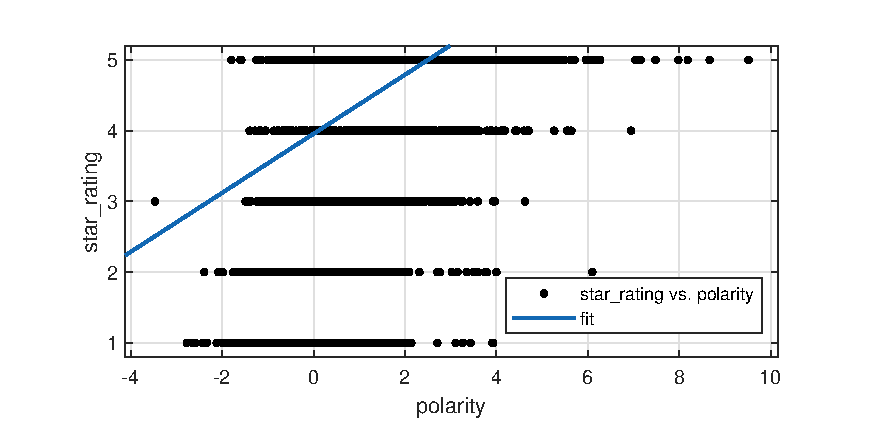
\includegraphics[width=\linewidth]{figures/pacifier/polarity_vs_star_rating.eps}
    \caption{star rating vs polarity}
    \label{fig:}
  \end{subfigure}%
  \begin{subfigure}{.5\textwidth}
    \centering
    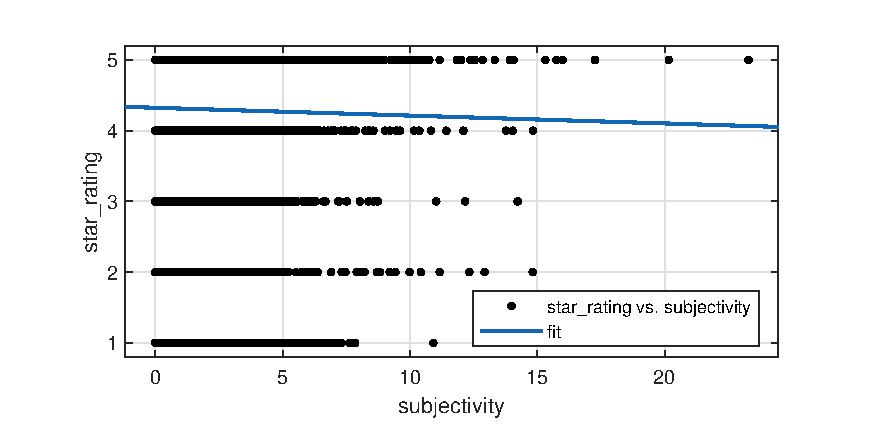
\includegraphics[width=\linewidth]{figures/pacifier/subjectivity_vs_star_rating.eps}
    \caption{star rating vs subjectivity}
    \label{fig:}
  \end{subfigure}
  \caption{the relation between polarity, subjectivity and star rating of the pacifier}
  \label{fig:}
\end{figure}
As \textbf{MATLAB} told us, the star rating, noted in $r$, is linearly related with customer's polarity $p$. And $r$ is unrelated with subjectivity of the customer $s$. For the hair dryer
\begin{equation*}
  \begin{aligned}
    r = 0.515 p + 3.652
  \end{aligned}
\end{equation*}
For the microwave
\begin{equation*}
  \begin{aligned}
    r = 0.5949 p + 2.969
  \end{aligned}
\end{equation*}
For the pacifier
\begin{equation*}
  \begin{aligned}
    r = 0.4172 p + 3.957
  \end{aligned}
\end{equation*}

\subsection{The influence among different star ratings and reviews}
\label{sec:The influence among different star ratings and reviews}

For customers, writing reviews and rating products are commonly not completely an individual behavior. For instance, if you see others giving bad comments to a product, you will tend to think that the product is not as good as the product it actually is. In finding how previous reviews and star ratings may infect a customer's view of a product, we made the following assumptions

\begin{enumerate}[\bfseries 1.]
\item Assume that the customer is only infected by previous reviews and star ratings. Customers may not be infected by the vendors, the shopping platforms, etc. The final star rating is decided by the customer's experience and other's ratings.
\item Assume that the customer is more convinced by the reviews whose star rating is close to his own star rating.
\item Assume the customer tend to read from the latest reviews rather than reviews far previous.
\item Assume the number of reviews a customer tends to see obeys normal distribution, and the average reviews a customer wants to see is 5. So that the user won't see a review which is created, for example, 1 year ago. When the reviews are created doesn't matter in this problem.
\end{enumerate}

According to the first 2 assumptions, we define the influence, to determine in what degree others' reviews may effect a customer's review. Because the reviews is linearly related with the star rating, we use star rating to represent the customers' attitude towards the product. We define
\begin{equation*}
  \begin{aligned}
    I = k_1 (R - \bar{R}) + k_2 (R - \bar{R}_{star})
  \end{aligned}
\end{equation*}
Whereas $I$ is the influence, $R$ is the star rating customer tend to give before seeing others reviews, $\bar{R}$ is the average star rating of product before the user gives a rating, which indicates the quality of a product at that time. $\bar{R}_{star}$ is the average of star rating the customer seen, $k_1$ and $k_2$ are constants.

We used object oriented programming of \textbf{MATLAB} to solve the problem. The source code of the program is in \textbf{Appendix}

In the program, we defined 2 classes: Customer and Product. Customers has properties like polarity and subjectivity, and product has reviews given by customers. We created the same amount of customers given by the data, set $k_1$ and $k_2$ to different values, then set the polarity and subjectivity of the created customers to the real customers' polarity and subjectivity. And let them to give star ratings of the product one by one in order.

Each customer will see random amount of previous reviews, and the star rating a customer finally give in the stars he may give before seeing the reviews plus the influence $I$

We carefully adjust the 2 constants, until the distribution of star ratings those customers gave is similar to the real star ratings in data.

We used the data of hair dryer. When we set $k_1=0.7$ and $k_2=0.13$, we found the data we manually created was quite similar with the real one. The following graph shows the distribution of star ratings and the difference between the real data and the data we created.

\begin{figure}[H]
  \centering
  \includegraphics[width=0.7\linewidth]{Q4picture/0.jpg}
  \caption{The distribution of star ratings of hair dryer}
  \label{fig:}
\end{figure}

Since the customers see random numbers of previous reviews and star ratings, to show our model is stable, we ran the program for 2 more times. And the outputs are almost the same.

\begin{figure}[H]
  \centering
  \begin{subfigure}{.5\textwidth}
    \centering
    \includegraphics[width=\linewidth]{Q4picture/1.jpg}
    \label{fig:}
  \end{subfigure}%
  \begin{subfigure}{.5\textwidth}
    \centering
    \includegraphics[width=\linewidth]{Q4picture/2.jpg}
    \label{fig:}
  \end{subfigure}
  \caption{The program gave us same result each time we ran}
  \label{fig:}
\end{figure}

Then we applied the same model to the pacifier and the microwave, and , surprisingly, we founded out that for different products, the 2 constants, $k_1$ and $k_2$, are the same.

That is probably because the 2 constants are properties of customers, and are not related to certain products, and the customers are the same. These 2 graphs show that our model fixed well on the microwave and pacifier as well.


\begin{figure}[H]
  \centering
  \begin{subfigure}{.5\textwidth}
    \centering
    \includegraphics[width=\linewidth]{Q4picture/microwave}
    \caption{The distribution of star ratings of microwave}
    \label{fig:}
  \end{subfigure}%
  \begin{subfigure}{.5\textwidth}
    \centering
    \includegraphics[width=\linewidth]{Q4picture/pacifier}
    \caption{The distribution of star ratings of pacifier}
    \label{fig:}
  \end{subfigure}
  \caption{Our model fits well on other products}
  \label{fig:}
\end{figure}

\subsection{Predict the future of the 3 products}

Since the data of star rating we created can successfully fit the real star ratings of all the 3 products, if we create more customers, we can predict their ratings as well.

Our assumptions is the same as before. And to ensure the future customers is the same as the customers we had known from data, we assume the polarity and subjectivity obey normal distribution.

We used the \textbf{Distribution Fitter} app in \textbf{MATLAB} to find the $\sigma$ and $\mu$ of the normal distribution polarity and subjectivity obeys. And we created future customers, whose polarity and subjectivity is generated from the 2 normal distribution we just known.

The rating customers gave before being influenced by other reviews are linearly dependent with their polarity. And the relation is already known in section \ref{sec:The influence among different star ratings and reviews}

For the hair dryers and the pacifier, we created 5000 future customers, and the distribution of their ratings are shown below

\begin{figure}[H]
  \centering
  \begin{subfigure}{.5\textwidth}
    \centering
    \includegraphics[width=\linewidth]{Q3picture/hair_dryer.jpg}
    \caption{The distribution of star ratings of hair dryer}
    \label{fig:}
  \end{subfigure}%
  \begin{subfigure}{.5\textwidth}
    \centering
    \includegraphics[width=\linewidth]{Q3picture/pacifier.jpg}
    \caption{The distribution of star ratings of pacifier}
    \label{fig:}
  \end{subfigure}
  \caption{The future star ratings our model predicted}
  \label{fig:}
\end{figure}

We can see that future customers tend to give 4 stars, and the reputation of the 2 products may stay unchanged.

But for the microwave, we created 500 future customers, and found out the future customers spoke highly of the microwave, compared to the customers we known from data. Less 1 star ratings are generated, more high star ratings appeared. This indicates that the microwave may has potential to success.
\begin{figure}[H]
  \centering
  \includegraphics[width=0.7\linewidth]{Q3picture/microwave.jpg}
  \caption{The future star ratings of microwave we predicted}
  \label{fig:}
\end{figure}



\section{Strengths and Weaknesses}
\subsection{Strengths}
\begin{itemize}
    \item First one...
    \item Second one ...
\end{itemize}

\subsection{Weaknesses}
\begin{itemize}
    \item Only one ...
 \end{itemize}


% 以下为信件/备忘录部分,不需要可自行去掉
% 如有需要可将整个 letter 环境移动到文章开头或中间
% 请在后一个花括号内填写信件(Letter)或备忘录(Memorandum)标题
\begin{letter}{Memorandum}
\begin{flushleft}  % 左对齐环境,无首行缩进
\textbf{To:} Heishan Yan\\
\textbf{From:} Team XXXXXXX\\
\textbf{Date:} October 1st, 2019\\
\textbf{Subject:} A better choice than MS Word: \LaTeX
\end{flushleft}

In the memo, we want to introduce you an alternate typesetting program to the prevailing MS Word: \textbf{\LaTeX}. In fact, the history of \LaTeX\ is even longer than that of MS Word. In 1970s, the famous computer scientist Donald Knuth first came out with a typesetting program, which named \TeX\ \ldots

Firstly, \ldots

Secondly, \ldots

Lastly, \ldots

According to all those mentioned above, it is really worth to have a try on \LaTeX! 
\end{letter}


% 参考文献,此处以 MLA 引用格式为例
\begin{thebibliography}{99}
\bibitem{1} Einstein, A., Podolsky, B., \& Rosen, N. (1935). Can quantum-mechanical description of physical reality be considered complete?. \emph{Physical review}, 47(10), 777.
\bibitem{2} \emph{A simple, easy \LaTeX\ template for MCM/ICM: EasyMCM}. (2018). Retrieved December 1, 2019, from\url{https://www.cnblogs.com/xjtu-blacksmith/p/easymcm.html}
\end{thebibliography}


% 以下为附录内容
% 如您的论文中不需要附录,请自行删除
\begin{subappendices}  % 附录环境

  \section{Appendix: The source code of our program used to creating customers and rate products}
  \noindent
Main.m
\lstset{
 basicstyle=\ttfamily,
 breaklines=true,
 columns=fixed,       
 numbers=left,                                        % 在左侧显示行号
 numberstyle=\tiny\color{gray},                       % 设定行号格式
 frame=single,                                          % 不显示背景边框
 backgroundcolor=\color[RGB]{245,245,244},            % 设定背景颜色
 keywordstyle=\color[RGB]{40,40,255},                 % 设定关键字颜色
 numberstyle=\footnotesize\color{darkgray},           
 commentstyle=\it\color[RGB]{0,96,96},                % 设置代码注释的格式
 stringstyle=\rmfamily\slshape\color[RGB]{128,0,0},   % 设置字符串格式
 showstringspaces=false,                              % 不显示字符串中的空格
 language=octave,                                        % 设置语言
}

\begin{lstlisting}
clc, clear

k1=0.7;
k2=0.13;

load('data.mat')
real_product = Product(star_rating, polarity, subjectivity);
real_products_in_total = size(real_product.reviews,1);

customers_index = 1:real_products_in_total;

virtual_product = Product(3,0,0.5);
for i = customers_index
    new_customer = Customer(virtual_product, star_rating(i,1), polarity(i,1), subjectivity(i,1), k1, k2);
    new_review = [new_customer.rating,new_customer.polarity,new_customer.subjectivity];
    new_virtual_product = Product([virtual_product.reviews(:,1);new_review(:,1)],[virtual_product.reviews(:,2);new_review(:,2)],[virtual_product.reviews(:,3);new_review(:,3)]);
    virtual_product = new_virtual_product;
end
virtual_ratings = virtual_product.reviews(2:real_products_in_total,1);
% plot(1:real_products_in_total-1, transpose(virtual_ratings),'*')
virtual_ratings_freq = [sum(virtual_ratings(:) <= 1);sum(virtual_ratings(:) == 2);sum(virtual_ratings(:) == 3);sum(virtual_ratings(:) == 4);sum(virtual_ratings(:) >= 5)];
real_ratings_freq = [sum(star_rating(:) <= 1);sum(star_rating(:) == 2);sum(star_rating(:) == 3);sum(star_rating(:) == 4);sum(star_rating(:) >= 5)];
error_of_ratings_freq = sum(abs(virtual_ratings_freq - real_ratings_freq));
bar([virtual_ratings_freq,real_ratings_freq])
legend('virtual ratings','real ratings')
xlabel('stars')
ylabel('numbers')
title(['k1=',num2str(k1),', k2=',num2str(k2),', error=', num2str(error_of_ratings_freq)])
\end{lstlisting}
\newpage
\noindent
Customer.m
\begin{lstlisting}
classdef Customer
    properties
        reviews_wants_to_see
        polarity
        subjectivity
        rating
        real_rating
        product
        k1
        k2
    end
    methods
        function obj = Customer(product, real_rating, real_polarity, real_subjectivity, k1, k2)
            obj.k1 = k1;
            obj.k2 = k2;
            obj.reviews_wants_to_see = round(max(0,normrnd(5,3)));
            obj.polarity = real_polarity;
            obj.subjectivity = real_subjectivity;
            obj.product = product;
            obj.real_rating = real_rating;
            obj.rating = rate(obj);
        end
        function influence_parameter = generateInfluenceParameter(obj)
            influence_parameter = 1;
        end
        function rating = rate(obj)
            total_number_of_reviews = size(obj.product.reviews, 1);
            numbers_of_reviews_being_seen = min(total_number_of_reviews, obj.reviews_wants_to_see);
            reviews_being_seen = obj.product.reviews(total_number_of_reviews - numbers_of_reviews_being_seen + 1:total_number_of_reviews,:);
            if size(reviews_being_seen,1) == 0
                reviews_being_seen = 0;
            end
            influence = (obj.k1*(obj.real_rating - obj.product.quality) + obj.k2 * numbers_of_reviews_being_seen * (obj.real_rating - mean(reviews_being_seen(:,1))));
            rating = round(influence + obj.product.quality);
        end  
    end
end
\end{lstlisting}
\newpage
\noindent
Product.m
\begin{lstlisting}
classdef Product
    properties
        quality
        reviews
    end
    
    methods
        function obj = Product(star_rating, polarity, subjectivity)
            obj.quality = mean(star_rating);
            obj.reviews = [star_rating polarity subjectivity];
        end
    end
end
\end{lstlisting}
\end{subappendices}

\end{document}  % 结束